%
%  =======================================================================
%  ····Y88b···d88P················888b·····d888·d8b·······················
%  ·····Y88b·d88P·················8888b···d8888·Y8P·······················
%  ······Y88o88P··················88888b·d88888···························
%  ·······Y888P··8888b···88888b···888Y88888P888·888·88888b·····d88b·······
%  ········888······"88b·888·"88b·888·Y888P·888·888·888·"88b·d88P"88b·····
%  ········888···d888888·888··888·888··Y8P··888·888·888··888·888··888·····
%  ········888··888··888·888··888·888···"···888·888·888··888·Y88b·888·····
%  ········888··"Y888888·888··888·888·······888·888·888··888··"Y88888·····
%  ·······························································888·····
%  ··························································Y8b·d88P·····
%  ···························································"Y88P"······
%  =======================================================================
% 
%  -----------------------------------------------------------------------
% Author       : 焱铭
% Date         : 2023-08-08 12:40:13 +0800
% LastEditTime : 2023-08-19 23:15:11 +0800
% Github       : https://github.com/YanMing-lxb/
% FilePath     : \YM-Beamer-Metropolis\YM-Beamer.tex
% Description  : 
%  -----------------------------------------------------------------------
%

\documentclass[compress,aspectratio=43,10pt,UTF8]{ctexbeamer} 
%默认字体12pt,编码使用UTF8,使用中文

\usetheme[progressbar=frametitle]{metropolis} 
% 使用metropolis主题,设置进度条在frametitle上显示
\useinnertheme{metropolis}
% \useoutertheme{infolines}
% \setbeamertemplate{headline}{} % 移除顶部导航栏
% \usecolortheme{custom}

\setbeamertemplate{footline}{%
  \begin{beamercolorbox}[wd=\paperwidth,ht=2.25ex,dp=1ex]{footlinecolor}
    \tiny
    \hspace*{1em} % 左边距
    \centering
    \insertshortauthor\hfill % 作者
    \insertshorttitle\hfill % 标题
    \colorbox{mDarkTeal}{\hspace*{4em}\textcolor{white}{\insertshortdate\hspace*{4em}
    \insertframenumber/\inserttotalframenumber\hspace*{1em}}} % 页码
  \end{beamercolorbox}%
}

\usepackage{appendixnumberbeamer}
\usepackage{latexsym,xcolor,multicol,multirow,booktabs,threeparttable,array,calligra,tabularray,calligra}
\usepackage[scale=2]{ccicons} % 使用ccicons宏包,用于排版Creative Commons图标

\usepackage{graphicx,pstricks,listings,stackengine}
\usepackage[labelformat=simple]{subcaption} % 使用subcaption宏包,设置子图标题格式为简单格式
\renewcommand{\thesubfigure}{(\alph{subfigure})} % 设置子图标题的序号格式为(a)、(b)等
\setbeamerfont{caption}{size=\scriptsize} % 设置caption的字体大小为scriptsize
\captionsetup[subfigure]{aboveskip=2pt, belowskip=2pt}% , width=36pt 设置子图标题的宽度 
\captionsetup[subfoat]{aboveskip=2pt, belowskip=2pt}
\captionsetup[figure]{aboveskip=3pt, belowskip=0pt} 
\captionsetup[table]{aboveskip=0pt, belowskip=6pt}

%语法高亮
% \usepackage{minted}

\usepackage{pgfplots} % 使用pgfplots宏包,用于绘制图表,使用dateplot库,用于绘制日期图表
\usepgfplotslibrary{dateplot}
\usepackage{hologo} % 使用hologo宏包,用于排版各种logo

\usepackage{amsmath, amsfonts, amssymb} %数学符号

\usepackage{hyperref}

\usepackage{xspace} %断行命令
\newcommand{\themename}{\textbf{\textsc{metropolis}}\xspace}

\graphicspath{{./Picture/}} % 图片所在位置





\title{YM Beamer Theme} %标题
\subtitle{毕业开题/答辩 or 组会报告} %副标题
\date{\today} %今天的日期
% \date{} %指定日期
\author{焱铭} %作者
\institute{桂林电子科技大学} %机构
\titlegraphic{\hfill
\includegraphics[height=1.5cm]{Guet-logo.pdf}} %插入logo


% ------------------------------------------------------------------------------------------
%     正文
% ------------------------------------------------------------------------------------------
\begin{document}

\maketitle %目录生成

\begin{frame}{目录}
	%		Table of contents 目录/大纲页
	%             自动实现对section的收集,并绘制成目录页
  \setbeamertemplate{section in toc}[sections numbered]
  \tableofcontents[hideallsubsections] % 隐藏subsection
\end{frame}




\section{课题背景}

\begin{frame}{用Beamer很高大上?}
    \begin{itemize}[<+-| alert@+>] % 当然,除了alert,手动在里面插 \pause 也行
        \item 该Beamer模板采用metropolis主题
        \item 中文支持请选择 Xe\LaTeX{} 编译选项
        \item 自用模板,可用于组会汇报、毕业答辩、复试。
    \end{itemize}
\end{frame}

\begin{frame}[allowframebreaks]{What is beamer?}
	Beamer 是一个用于创建演示文稿 LaTeX 的文档类。它同时支持\LaTeX + dvips、\hologo{pdfLaTeX}、\hologo{LuaLaTeX}以及\hologo{XeLaTeX}。它的名称取自德语词汇 Beamer(pseudo-anglicism),意思是影像演示。
	
	Beamer文档类并不是最早开发出的\LaTeX 演示文稿工具。2003年2月,Till Tantau为其博士论文答辩编写了beamer包,并于一个月之后发布在CTAN上。
	
	作为LaTeX的一个文档类,Beamer文档和\LaTeX 文档一样都是纯文本文件。且beamer兼容\LaTeX 常见的命令,和其他宏包的兼容性良好。
	
	当然也有支持Beamer语法的图形界面,如AUCTEX和LyX。
	
	Beamer也可以通过使用兼容包来支持其他LaTeX演示文稿宏包的语法,包括 Prosper和Foils。
	
	Beamer默认生成PDF文件用于演示,其动态效果依靠创建多页幻灯片实现。
	
	若要打印出每张幻灯片的最终效果用于分发给听众,需开启handout选项;想要在一张纸上打印多页幻灯片,需要用pgfpages宏包;也可以输出适合印刷在A4或者标准信纸上的文档效果。
	
	'frame'的标题将变为段落的标题,不再包括原有的外观主题,同时保证了原有章节结构不被破坏——这就可以方便的输出演讲的提纲。
	
	Beamer的一些功能是依赖于PGF的。
	
	以上介绍来自WiKipedia。\footnote{https://zh.wikipedia.org/wiki/Beamer\_(LaTeX)}
	
	关于如何自制一份beamer,请浏览\href{https://zhuanlan.zhihu.com/p/423443762}{用LaTeX创建一个Beamer},可以关注专栏,及时获得推动与建议。
\end{frame}

\begin{frame}[fragile]{如何提供一份讲义}
	你可以给你的观众一张幻灯片的印刷版。只需使用handout选项创建文档的一个版本,就不会使用覆盖图:
\begin{lstlisting}[language=TeX]
\documentclass[handout]{beamer}
\usepackage{pgfpages}
\pgfpagesuselayout{4 on 1}[a4paper,border shrink=5mm,landscape]
\end{lstlisting}
这将在A4纸上横向打印四张幻灯片。通过指定以下代码行,可以在纵向模式下获得更大的打印,每页两张幻灯片:
\begin{lstlisting}[language=TeX]
\pgfpagesuselayout{2 on 1}[a4paper,border shrink=5mm]
\end{lstlisting}
使用这一功能必须加载pgf宏包,并启用pgfpages选项,这是pgf宏包附带的一个实用宏包。
\end{frame}


\section{研究现状}

\subsection{如何更好地做Beamer}

\begin{frame}{Why Beamer}
    \begin{itemize}
        \item \LaTeX 广泛用于学术界,期刊会议论文模板
    \end{itemize}
    \begin{table}[h]
        \centering
        \begin{tabular}{c|c}
            Microsoft\textsuperscript{\textregistered}  Word & \LaTeX \\
            \hline
            文字处理工具 & 专业排版软件 \\
            容易上手,简单直观 & 容易上手 \\
            所见即所得 & 所见即所想,所想即所得 \\
            高级功能不易掌握 & 进阶难,但一般用不到 \\
            处理长文档需要丰富经验 & 和短文档处理基本无异 \\
            花费大量时间调格式 & 无需担心格式,专心作者内容 \\
            公式排版差强人意 & 尤其擅长公式排版 \\
            二进制格式,兼容性差 & 文本文件,易读、稳定 \\
            付费商业许可 & 自由免费使用 \\
        \end{tabular}
    \end{table}
\end{frame}

\begin{frame}{如何使用块}
    \begin{block}{块的名称}
        \begin{itemize}
            \item A
            \item B
        \end{itemize}
    \end{block}	
\end{frame}

\begin{frame}{Blocks}
    三种不同的块环境是预定义的,并且可以使用可选的背景颜色设置样式。

    \begin{columns}[T,onlytextwidth]
        \column{0.5\textwidth}
        \begin{block}{Default}
            Block content.
        \end{block}

        \begin{alertblock}{Alert}
            Block content.
        \end{alertblock}

        \begin{exampleblock}{Example}
            Block content.
        \end{exampleblock}

        \column{0.5\textwidth}

        \metroset{block=fill}

        \begin{block}{Default}
            Block content.
        \end{block}

        \begin{alertblock}{Alert}
            Block content.
        \end{alertblock}

        \begin{exampleblock}{Example}
            Block content.
        \end{exampleblock}

    \end{columns}
\end{frame}

\begin{frame}{排版举例}
	
	\begin{block}{无编号公式}
        \begin{equation*}
            J(\theta) = \mathbb{E}_{\pi_\theta}[G_t] = \sum_{s\in\mathcal{S}} d^\pi (s)V^\pi(s)=\sum_{s\in\mathcal{S}} d^\pi(s)\sum_{a\in\mathcal{A}}\pi_\theta(a|s)Q^\pi(s,a)
        \end{equation*}
    \end{block}
    \begin{block}{多行多列公式\footnotemark[1]}
        % 使用 & 分隔
        \begin{align}
            Q_\mathrm{target}&=r+\gamma Q^\pi(s^\prime, \pi_\theta(s^\prime)+\epsilon)\\
            \epsilon&\sim\mathrm{clip}(\mathcal{N}(0, \sigma), -c, c)\nonumber
        \end{align}
    \end{block}
    \footnotetext[1]{如果公式中有文字出现,请用 $\backslash$mathrm\{\} 或者 $\backslash$text\{\} 包含,不然就会变成 $clip$,在公式里看起来比 $\mathrm{clip}$ 丑非常多。}
\end{frame}

\begin{frame}
    \begin{block}{编号多行公式}
        % Taken from Mathmode.tex
        \begin{multline}
            A=\lim_{n\rightarrow\infty}\Delta x\left(a^{2}+\left(a^{2}+2a\Delta x+\left(\Delta x\right)^{2}\right)\right.\label{eq:reset}\\
            +\left(a^{2}+2\cdot2a\Delta x+2^{2}\left(\Delta x\right)^{2}\right)\\
            +\left(a^{2}+2\cdot3a\Delta x+3^{2}\left(\Delta x\right)^{2}\right)\\
            +\ldots\\
            \left.+\left(a^{2}+2\cdot(n-1)a\Delta x+(n-1)^{2}\left(\Delta x\right)^{2}\right)\right)\\
            =\frac{1}{3}\left(b^{3}-a^{3}\right)
        \end{multline}
    \end{block}
\end{frame}

\begin{frame}{图形与分栏}
    % From thuthesis user guide.
    \begin{minipage}[c]{0.3\linewidth}
        \psset{unit=0.8cm}
        \begin{pspicture}(-1.75,-3)(3.25,4)
            \psline[linewidth=0.25pt](0,0)(0,4)
            \rput[tl]{0}(0.2,2){$\vec e_z$}
            \rput[tr]{0}(-0.9,1.4){$\vec e$}
            \rput[tl]{0}(2.8,-1.1){$\vec C_{ptm{ext}}$}
            \rput[br]{0}(-0.3,2.1){$\theta$}
            \rput{25}(0,0){%
            \psframe[fillstyle=solid,fillcolor=lightgray,linewidth=.8pt](-0.1,-3.2)(0.1,0)}
            \rput{25}(0,0){%
            \psellipse[fillstyle=solid,fillcolor=yellow,linewidth=3pt](0,0)(1.5,0.5)}
            \rput{25}(0,0){%
            \psframe[fillstyle=solid,fillcolor=lightgray,linewidth=.8pt](-0.1,0)(0.1,3.2)}
            \rput{25}(0,0){\psline[linecolor=red,linewidth=1.5pt]{->}(0,0)(0.,2)}
%           \psRotation{0}(0,3.5){$\dot\phi$}
%           \psRotation{25}(-1.2,2.6){$\dot\psi$}
            \psline[linecolor=red,linewidth=1.25pt]{->}(0,0)(0,2)
            \psline[linecolor=red,linewidth=1.25pt]{->}(0,0)(3,-1)
            \psline[linecolor=red,linewidth=1.25pt]{->}(0,0)(2.85,-0.95)
            \psarc{->}{2.1}{90}{112.5}
            \rput[bl](.1,.01){C}
        \end{pspicture}
    \end{minipage}\hspace{1cm}
    \begin{minipage}{0.5\linewidth}
        \medskip
        %\hspace{2cm}
        \begin{figure}[h]
            \centering
            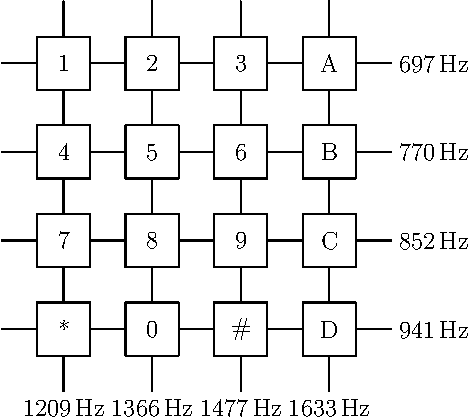
\includegraphics[height=.4\textheight]{dtmf.pdf}
        \end{figure}
    \end{minipage}
\end{frame}

\begin{frame}{Line plots}
  \begin{figure}
    \begin{tikzpicture}
      \begin{axis}[
        mlineplot,
        width=0.9\textwidth,
        height=6cm,
      ]

        \addplot {sin(deg(x))};
        \addplot+[samples=100] {sin(deg(2*x))};

      \end{axis}
    \end{tikzpicture}
  \end{figure}
\end{frame}

\begin{frame}{Bar charts}
  \begin{figure}
    \begin{tikzpicture}
      \begin{axis}[
        mbarplot,
        xlabel={Foo},
        ylabel={Bar},
        width=0.9\textwidth,
        height=6cm,
      ]

      \addplot plot coordinates {(1, 20) (2, 25) (3, 22.4) (4, 12.4)};
      \addplot plot coordinates {(1, 18) (2, 24) (3, 23.5) (4, 13.2)};
      \addplot plot coordinates {(1, 10) (2, 19) (3, 25) (4, 15.2)};

      \legend{lorem, ipsum, dolor}

      \end{axis}
    \end{tikzpicture}
  \end{figure}
\end{frame}



\begin{frame}[fragile]{\LaTeX{} 环境命令举例}
    \begin{minipage}{0.5\linewidth}
\begin{lstlisting}[language=TeX]
\begin{itemize}
  \item A \item B
  \item C
  \begin{itemize}
    \item C-1
  \end{itemize}
\end{itemize}
\end{lstlisting}
    \end{minipage}\hspace{1cm}
    \begin{minipage}{0.3\linewidth}
        \begin{itemize}
            \item A
            \item B
            \item C
            \begin{itemize}
                \item C-1
            \end{itemize}
        \end{itemize}
    \end{minipage}
    \medskip
    \pause
    \begin{minipage}{0.5\linewidth}
\begin{lstlisting}[language=TeX]
\begin{enumerate}
  \item 巨佬 \item 大佬
  \item 萌新
  \begin{itemize}
    \item[n+e] 瑟瑟发抖
  \end{itemize}
\end{enumerate}
\end{lstlisting}
    \end{minipage}\hspace{1cm}
    \begin{minipage}{0.3\linewidth}
        \begin{enumerate}
            \item 巨佬
            \item 大佬
            \item 萌新
            \begin{itemize}
                \item[n+e] 瑟瑟发抖
            \end{itemize}
        \end{enumerate}
    \end{minipage}
\end{frame}

\begin{frame}[fragile]{\LaTeX{} 数学公式}
    \begin{columns}
        \begin{column}{.55\textwidth}
\begin{lstlisting}[language=TeX]
$V = \frac{4}{3}\pi r^3$

\[
  V = \frac{4}{3}\pi r^3
\]

\begin{equation}
  \label{eq:vsphere}
  V = \frac{4}{3}\pi r^3
\end{equation}
\end{lstlisting}
        \end{column}
        \begin{column}{.4\textwidth}
            $V = \frac{4}{3}\pi r^3$
            \[
                V = \frac{4}{3}\pi r^3
            \]
            \begin{equation}
                \label{eq:vsphere}
                V = \frac{4}{3}\pi r^3
            \end{equation}
        \end{column}
    \end{columns}
    \begin{itemize}
        \item 更多内容请看 \href{https://zh.wikipedia.org/wiki/Help:数学公式}{\color{purple}{这里}}
    \end{itemize}
\end{frame}

\begin{frame}[fragile]
    \begin{columns}
        \column{.6\textwidth}
\begin{lstlisting}[language=TeX]
    \begin{table}[htbp]
      \caption{编号与含义}
      \label{tab:number}
      \centering
      \begin{tabular}{cl}
        \toprule
        编号 & 含义 \\
        \midrule
        1 & 4.0 \\
        2 & 3.7 \\
        \bottomrule
      \end{tabular}
    \end{table}
    公式~(\ref{eq:vsphere}) 的
    编号与含义请参见
    表~\ref{tab:number}。
\end{lstlisting}
        \column{.4\textwidth}
        \begin{table}[htpb]
            \centering
            \caption{编号与含义}
            \label{tab:number}
            \begin{tabular}{cl}\toprule
                编号 & 含义 \\\midrule
                1 & 4.0\\
                2 & 3.7\\\bottomrule
            \end{tabular}
        \end{table}
        \normalsize 公式~(\ref{eq:vsphere})的编号与含义请参见表~\ref{tab:number}。
    \end{columns}
\end{frame}


\begin{frame}{作图}
    \begin{itemize}
        \item 矢量图 eps, ps, pdf
        \begin{itemize}
            \item METAPOST, pstricks, pgf $\ldots$
            \item Xfig, Dia, Visio, Inkscape $\ldots$
            \item Matlab / Excel 等保存为 pdf
        \end{itemize}
        \item 标量图 png, jpg, tiff $\ldots$
        \begin{itemize}
            \item 提高清晰度,避免发虚
            \item 应尽量避免使用
        \end{itemize}
    \end{itemize}
    \begin{figure}[htpb]
        \centering
        
\includegraphics[width=0.2\linewidth]{Guet-logo.pdf}
        \caption{这个校徽就是矢量图}
    \end{figure}
\end{frame}

{\setbeamercolor{palette primary}{fg=black, bg=yellow}
\begin{frame}[standout]
  Questions?
\end{frame}
}

\section{计划进度}
\begin{frame}
    \begin{itemize}
        \item 一月:完成文献调研
        \item 二月:复现并评测各种Beamer主题美观程度
        \item 三、四月:美化GUET Beamer主题
        \item 五月:论文撰写
    \end{itemize}
\end{frame}

\begin{frame}{参考文献引用示例}
    参考文献引用 \cite{knuth92,ConcreteMath,Simpson,Er01,greenwade93}
  \end{frame}

\section{参考文献}

\begin{frame}[allowframebreaks]
    \bibliography{demo.bib}
    % \bibliographystyle{alpha}
    \bibliographystyle{abbrv}
    % 如果参考文献太多的话,可以像下面这样调整字体:
    % \tiny\bibliographystyle{alpha}
\end{frame}

\begin{frame}
    \begin{center}
        {\Huge\calligra Thanks!}
    \end{center}
\end{frame}

\end{document}
